\documentclass[12pt,fleqn]{article}
\usepackage{amsmath,epsf,times,zed-csp,fancyhdr,verbatim,graphicx,color}
\usepackage{breqn}
\setlength{\oddsidemargin}{0in}
\setlength{\evensidemargin}{0in}
\setlength{\topmargin}{-1.0in}
\setlength{\textheight}{8.5in}
\setlength{\headheight}{1.0in}
\setlength{\textwidth}{6.5in}

\pagestyle{fancy}

\lhead{\sc Models of Software Systems: Midterm Exam}
\cfoot{\thepage}

\begin{document}

\title{\sc Midterm Exam}
\author{Models of Software Systems\\Instructor: Dawn McLaughlin}
\date{October 19, 2018}
\maketitle

\noindent \textsc{Important Notes:}

\begin{itemize}
\item This exam should have 13 pages, including this cover sheet. If it does not, please notify your instructor(s) immediately.
\item You may use your books and notes for
this exam, but \textsc{you may not discuss this exam with anyone.} If you have questions about the exam, feel free to ask me privately by e-mail.
\item Exams should be submitted via Canvas by 7:00\textsc{am} Eastern (Daylight) time on Monday, October 22, 2018. 
\end{itemize}


\clearpage


\section*{\sc Part 1:}

Consider the following definition of trees that expands on the variety already seen on homework assignments:

$$TREE ::= leaf \langle\langle \nat \rangle\rangle | binary\_node \langle\langle \nat \cross TREE \cross TREE \rangle\rangle | ternary\_node \langle\langle \nat \cross TREE \cross TREE \cross TREE\rangle\rangle$$

It says that a tree is either a leaf which has a numeric value, it is a binary node which has a numeric value and has two subtrees, or it is a ternary node which has a numeric value and has three subtrees.

Here are some examples of trees:

\begin{center}
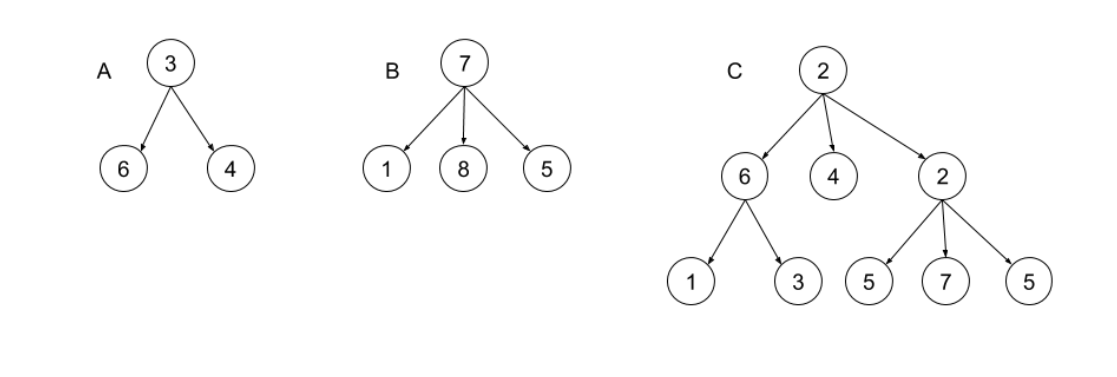
\includegraphics[width=4.5in]{trees.png}
\end{center}

Tree A has two leaves and one binary node; tree B has three leaves and one ternary node; tree C has six leaves, one binary node, and two ternary nodes.

Tree A can be described as $$binary\_node(3,leaf(6),leaf(4))$$ and tree B as $$ternary\_node(7,leaf(1),leaf(8),leaf(5))$$.

\begin{enumerate}
\item Give the description of tree C in the same format. [3 points]
\end{enumerate}

%-------------------------------------------
% Your answer goes here
%-------------------------------------------

\textcolor{blue}{
  $$ternary\_node(2,binary\_node(6,leaf(1),leaf(3)),leaf(4),ternary\_node(2,leaf(5),leaf(7),leaf(5)))$$
  }
%-------------------------------------------

\clearpage

Now consider the following function definitions:

\begin{axdef}
leaves : TREE \rightarrow \nat\\
nodes : TREE \rightarrow \nat\\
weight : TREE \rightarrow \nat
\where
\forall t_1, t_2, t_3:TREE@\forall n:\nat@\\ 
~\\
\quad leaves(leaf(n)) = 1 \land\\
\quad leaves(binary\_node(n,t_1,t_2)) = leaves(t_1) + leaves(t_2) \land\\
\quad leaves(ternary\_node(n,t_1,t_2,t_3)) = leaves(t_1) + leaves(t_2) + leaves(t_3) \land\\
~\\ 
\quad nodes(leaf(n)) = 0 \land\\
\quad nodes(binary\_node(n,t_1,t_2)) = 1 + nodes(t_1) + nodes(t_2) \land\\
\quad nodes(ternary\_node(n,t_1,t_2,t_3)) = 1 + nodes(t_1) + nodes(t_2) + nodes(t_3) \land\\
~\\ 
\quad weight(leaf(n)) = n \land\\
\quad weight(binary\_node(n,t_1,t_2)) = n + weight(t_1) + weight(t_2) \land\\
\quad weight(ternary\_node(n,t_1,t_2,t_3)) = n + weight(t_1) + weight(t_2) + weight(t_3)
\end{axdef}

\begin{enumerate}
\item[2.] The above definition of $nodes$ counts all nodes in the tree. Write axiomatic definitions for functions $binary\_nodes$ and $ternary\_nodes$ that count only the binary and ternary nodes of the tree, respectively. You may give one axiomatic definition for both functions, as was done for $leaves$, $nodes$, and $weight$, above, or you can do two separate axiomatic definitions, as you prefer. [2 $\times$ 5 = 10 points]

%-------------------------------------------
% Your answer goes here
%-------------------------------------------


%-------------------------------------------

\clearpage

\item[3.] Consider the following sets and predicates about these trees:

\begin{center}
\begin{tabular}{lp{4in}}
$TREE$ & the set of all trees\\
$three\_heavy(t)$ & $t$ is $three\_heavy$ if and only if it has strictly more ternary nodes than binary nodes (it must have at least one ternary node to be $three\_heavy$)\\
$two\_heavy(t)$ & $t$ is $two\_heavy$ if and only if it has strictly more binary nodes than ternary nodes (it must have at least one binary node to be $two\_heavy$)\\
$balanced(t)$ & $t$ is $balanced$ if and only if it has the same number of binary and ternary nodes (including none of either)
\end{tabular}
\end{center}

Using these predicates and the functions defined above, translate the following sentences about trees into predicate logic (note that some of the sentences may be false according to the definitions of the predicates). You may use standard arithmetic relations and functions (such as $<$, $>$, $\max$, $\min$, etc.), as required:

\begin{enumerate}
\item[a.] [3 points] A tree is $three\_heavy$ if and only if it is a leaf or has more ternary nodes than binary nodes. 

%-------------------------------------------
% Your answer goes here
%-------------------------------------------
\vspace{1in} %this line can be deleted when you enter your answer

%-------------------------------------------
\item[b.] [3 points] Every $three\_heavy$ tree $weigh$s more than some $two\_heavy$ tree. 

%-------------------------------------------
% Your answer goes here
%-------------------------------------------
\vspace{1in} %this line can be deleted when you enter your answer

%-------------------------------------------
\item[c.] [3 points] Some $three\_heavy$ tree $weigh$s more than every $two\_heavy$ tree. 

%-------------------------------------------
% Your answer goes here
%-------------------------------------------
\vspace{1in} %this line can be deleted when you enter your answer

%-------------------------------------------
\item[d.] [3 points] The immediate subtrees of any $balanced$ tree are either all $balanced$ or all have the same $weight$. 

%-------------------------------------------
% Your answer goes here
%-------------------------------------------
\vspace{1in} %this line can be deleted when you enter your answer

%-------------------------------------------
\end{enumerate}

\clearpage

\item[4.] Prove the following by structural induction: [15 points]
$$\forall t:TREE@nodes(t) = binary\_nodes(t) + ternary\_nodes(t)$$


\end{enumerate}

\clearpage

\section*{\sc Part 2:}

The following quadruple defines a state machine that models the (imaginary) Queequeg brand ``AutoBarista Mini'' coffee machine:

\begin{equation*}\begin{split}
\mathrm{Auto}&\mathrm{BaristaMini} = \{\\
&[ espresso : \{ 1, 2 \}, milk : \{ 0, 1 \} ],\\
&\{ s: S | espresso = 1 \wedge milk = 1 \},\\
&\{ e\_button, m\_button, d\_button\},\\
&\{(s,a,s'): S\times A\times S | \\
&\begin{split}
~~~~~&a = e\_button \Rightarrow (s'(milk)=s(milk) \wedge s'(espresso)\neq s(espresso) )\\
&\wedge\\
&a = m\_button \Rightarrow (s(milk)=1 \wedge s'(milk)=0 \wedge s'(espresso)=s(espresso))\\
&\wedge\\
&a = d\_button \Rightarrow (s'(milk)=1 \wedge s'(espresso)=1)
\end{split}\\
&\}\\
&\color{white}\mathrm{BaristaMini} = \color{black}\}
\end{split}\end{equation*}

Answer each of the following questions with respect to the above model.

\vspace*{2ex}

{\em Definitions:\\[2ex]
A cappuccino consists of steamed milk plus espresso.\\[1ex]
The terms ``single'' and ``double'' refer to the number of shots of espresso a beverage contains.}

\clearpage

\begin{enumerate}
\item Draw a transition diagram for $\mathrm{AutoBaristaMini}$. You may name individual states if you wish. For each state, be sure to indicate clearly the values of all state variables. Don't forget to label transitions. [15 points]
%-------------------------------------------
% Your answer goes here
%
% You may produce the diagram directly in
% \LaTeX if you wish, though this approach
% is not recommended, as it would likely be
% very time-consuming.
%
% Images should be included in the PDF of
% your submission. The commands to include
% graphics are as follows:
%
% includegraphics[scale=1.0]{file_name.extension}
%
% where the value for scale is a magnification 
% amount (useful if the image is too big - just
% set to the value less than 1)
%
% Both JPG and PNG formats should work without
% any hassle.
%
% Please check to make sure that the image
% as it appears in the PDF is correct and
% easy to read.
%
%-------------------------------------------

  \textcolor{blue}{It took me a long time to figure out what the states meant in the machine, after reaching
    out a few times to Dawn and by looking at the other questions, the best I could come with is that the state variables represent the user selection from milk and number of espresso shots.\\
\\
  To avoid cluttering the diagram with labels, I decided to color code the arrows, I could also have used arrows on both ends of the action line.}
  

\begin{center}
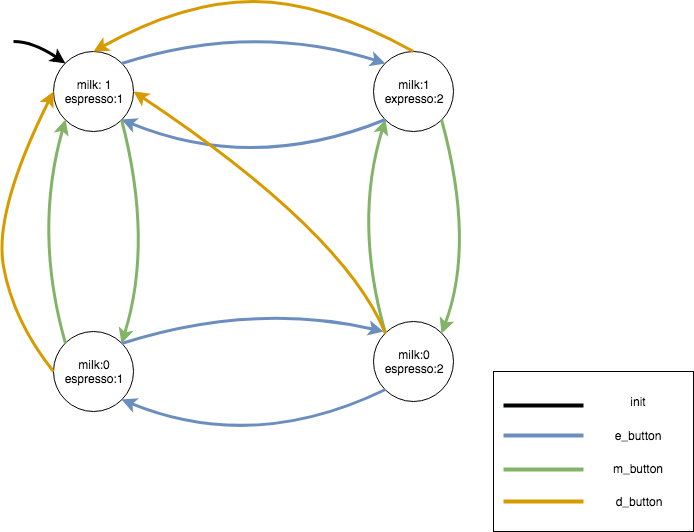
\includegraphics[width=6in]{BaristaMini.png}
\end{center}
%-------------------------------------------

\clearpage

\item Do each of the following:
\begin{enumerate}
\item Rewrite the set $\delta$ by enumeration (i.e., list all the triples). You may use the names you assigned to states in question (1) if you wish.  [5 points]

%-------------------------------------------
% Your answer goes here
%-------------------------------------------
  \textcolor{blue}{
    $\delta = ($\\
    $\{capuccino\_single\_shot, e\_button, capuccino\_double\_shot\},$ \\
    $\{capuccino\_single\_shot, m\_button, single\_shot\},$ \\
    $\{capuccino\_single\_shot, d\_button, capuccino\_single\_shot\},$ \\
    $\{capuccino\_double\_shot, m\_button, double\_shot\},$ \\
    $\{capuccino\_double\_shot, d\_button, capuccino\_single\_shot\},$ \\
    $\{capuccino\_double\_shot, e\_button, capuccino\_single\_shot\},$ \\
    $\{double\_shot, d\_button, capuccino\_single\_shot\},$ \\
    $\{double\_shot, e\_button, single\_shot\},$ \\
    $\{single\_shot, d\_button, capuccino\_single\_shot\},$ \\
    $\{single\_shot, e\_button, double\_shot\},$ \\
    $)$ \\
  }
%-------------------------------------------


\item Give the pre- and post-conditions of each action. [3 $\times$ 5 = 15 points]
\end{enumerate}

%-------------------------------------------
% Your answer goes here
%-------------------------------------------
\textcolor{blue}{
  $e\_button$ makes espresso toggle between 1 and 2 shots and keeps milk selection the same. \\
  $e\_button()$ \\
  $\textbf{pre:} true$  \\
  $\textbf{post:}$ (espresso = 1 $\implies$ (expresso' = 2 $\land$ milk' = milk)) $\land$ \\
                   (espresso = 2 $\implies$ (expresso' = 1 $\land$ milk' = milk)) \\
  \\
  $m\_button$ is only allowed if milk = 1, this threw me off a little bit but is what I was able to interpret from the state machine definition. It disables the milk.\\
  $m\_button()$ \\
  $\textbf{pre:} milk = 1$  \\
  $\textbf{post}:$ milk' = 0 $\land$ espresso' = espresso \\
  \\
  $d\_button()$ \\
  $\textbf{pre:} true$  \\
  \textbf{post:} milk' = 1 $\land$ espresso' = 1 \\}

%-------------------------------------------

\clearpage

\item Answer each of the following: [5 $\times$ 1 = 5 points]
\begin{enumerate}
\item Assuming that the $\mathrm{AutoBaristaMini}$ supplies a coffee cup each time $d\_button$ is pressed and it dispenses the selected drink, is it possible to get an empty cup from the machine?

%-------------------------------------------
% Your answer goes here
%-------------------------------------------
\textcolor{blue}{Based on the provided allowed variable values for espresso and milk that we can extract from the states definition ``$[ espresso : \{ 1, 2 \}, milk : \{ 0, 1 \} ]$''  it is not possible because you have to get either 1 or 2 shots of espreseo, meaning, it is not possible to select 0 shots and only get milk or nothing. }  
%-------------------------------------------


\item Give an informal explanation of what the $e\_button$ action does, in terms that an actual user of the machine would understand, i.e., without referring to the formal model.

%-------------------------------------------
% Your answer goes here
%-------------------------------------------
\textcolor{blue}{Toggle the number of espresso shots between 1 and 2.}
%-------------------------------------------


\item Give an informal explanation of what the $m\_button$ action does, in terms that an actual user of the machine would understand, i.e., without referring to the formal model.

%-------------------------------------------
% Your answer goes here
%-------------------------------------------
\textcolor{blue}{Disables milk, it is important to mention that it is not possible to enable it back without pressing $d\_button$ first.}
%-------------------------------------------


\item How many different drinks can $\mathrm{AutoBaristaMini}$ make?

%-------------------------------------------
% Your answer goes here
%-------------------------------------------
\textcolor{blue}{4, $\{single\_shot, double\_shot, cappuccino\_single\_shot, capuccino\_double\_shot\}$ there's a state for each drink.}
%-------------------------------------------


\item Give the event-based trace of the execution in which a double espresso, a single cappuccino, and a double cappuccino are dispensed, in that order.

%-------------------------------------------
% Your answer goes here
%-------------------------------------------
  \textcolor{blue}{The question is asking for a single execution: \\
    $<m\_button, e\_button, d\_button, d\_button, e\_button, d\_button>$
  }  
%-------------------------------------------
\end{enumerate}

\clearpage

\item Give an FSP specification of $\mathrm{AutoBaristaMini}$. [20 points]

%-------------------------------------------
% Your answer goes here
%-------------------------------------------
\begin{verbatim}
\color{blue}
//---------------------------------------------------
//  AutoBarista Mini
//---------------------------------------------------
//
//=====================
// Process Definitions
//=====================
//
// Autobarista starts in capuccino state
//
AUTO_BARISTA_MINI = CAPUCCINO_SINGLE_SHOT,
//
CAPUCCINO_SINGLE_SHOT = (
 e_button -> CAPUCCINO_DOUBLE_SHOT
 |m_button -> SINGLE_SHOT
 |d_button -> CAPUCCINO_SINGLE_SHOT 
),

CAPUCCINO_DOUBLE_SHOT = (
e_button -> CAPUCCINO_SINGLE_SHOT
 |m_button -> DOUBLE_SHOT
 |d_button -> CAPUCCINO_SINGLE_SHOT
),

SINGLE_SHOT = (
  d_button -> CAPUCCINO_SINGLE_SHOT
 |e_button -> CAPUCCINO_DOUBLE_SHOT
),

DOUBLE_SHOT = (
  d_button -> CAPUCCINO_SINGLE_SHOT
 |e_button -> CAPUCCINO_DOUBLE_SHOT
).
\end{verbatim}

\begin{center}
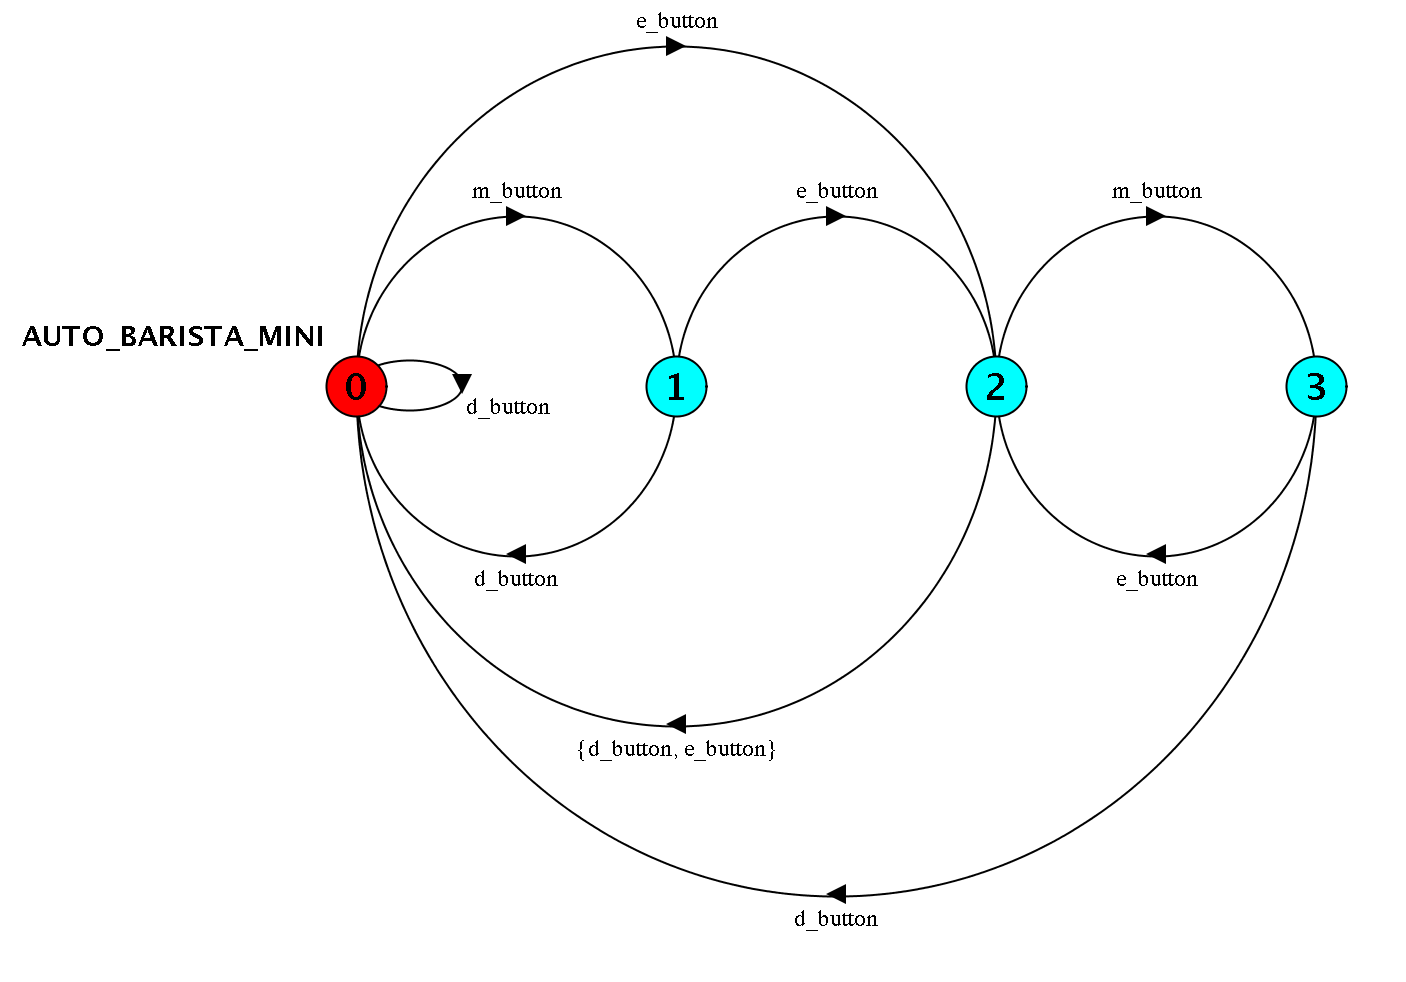
\includegraphics[width=6in]{fps_machine.png}
\end{center}
%-------------------------------------------

\clearpage

\item Consider the following additional behaviour of a more advanced model, the ``AutoBarista Eco'': The machine has a maximum stock of 100 cups. Each time it dispenses a drink, the user can put in their own reusable cup or the machine will automatically dispense a cup if no reusable cup is put in. When the machine is out of cups, it will not dispense a drink when no reusable cup is present. The act of adding more cups does not modify the drink that has been selected to be dispensed. The machine will always dispense a drink if a reusable cup has been inserted.

Here are the updated specifications of $S$, $I$, and $A$ for $\mathrm{AutoBaristaEco}$:
\begin{equation*}\begin{split}
S &= [ espresso :\{ 1, 2 \}, milk : \{ 0, 1 \}, cups : 0..100 ]\\
I &= \{ s: S | espresso = 1 \land milk = 1 \land cups = 100 \}\\
A &= \{ e\_button, m\_button, d\_button\}
\end{split}\end{equation*}

The pre- and post-conditions for $e\_button$ and $m\_button$ for $\mathrm{AutoBaristaEco}$ differ from those for $\mathrm{AutoBaristaMini}$ only by adding $cups^\prime = cups$ to the post-condition in each case.

Give the pre- and post-conditions for the $d\_button$ action of $\mathrm{AutoBaristaEco}$.

Model the reusable cup as an input: the input should be $true$ if a reusable cup has been inserted, $false$ if no cup has been inserted. [5 points]

%-------------------------------------------
% Your answer goes here
%-------------------------------------------


%-------------------------------------------

\clearpage

\section*{\sc Part 3:}

The AutoBarista Mini and Eco are limited-functionality, lower-end models in the Queequeg line of coffee machines. Their basic model is the AutoBarista, which is currently in the process of being re-engineered.

The AutoBarista is capable of producing drinks containing 0, 1, or 2 shots of espresso, with or without steamed milk, and in drinks containing steamed milk, with or without a shot of flavour syrup (syrup is not available for drinks containing only espresso). The machine offers a choice of three different syrups. There are thus a total of 14 different drinks the machine can produce. \\
\begin{center}
  \color{blue}
\begin{tabular}{ c c c c}
       & expresso & milk & flavour \\ 
 1     & $no\_shot$ & $yes\_milk$ & $no\_flavour$ \\  
 2     & $no\_shot$ & $yes\_milk$ & $flavour\_1$ \\
 3     & $no\_shot$ & $yes\_milk$ & $flavour\_2$ \\
 4     & $no\_shot$ & $yes\_milk$ & $flavour\_3$ \\
 5     & $one\_shot$ & $yes\_milk$ & $no\_flavour$ \\  
 6     & $one\_shot$ & $yes\_milk$ & $flavour\_1$ \\
 7     & $one\_shot$ & $yes\_milk$ & $flavour\_2$ \\
 8     & $one\_shot$ & $yes\_milk$ & $flavour\_3$ \\
 9     & $two\_shots$ & $yes\_milk$ & $no\_flavour$ \\  
 10    & $two\_shots$ & $yes\_milk$ & $flavour\_1$ \\
 11    & $two\_shots$ & $yes\_milk$ & $flavour\_2$ \\
 12    & $two\_shots$ & $yes\_milk$ & $flavour\_3$ \\
 13    & $one\_shot$ & $no\_milk$  & $no\_flavour$ \\
 14    & $two\_shots$ & $no\_milk$ & $no\_flavour$ \\
 \end{tabular}
\end{center}

\begin{enumerate}
\item[1.] Complete the following state space schema for the $\mathrm{AutoBarista}$ by supplying an appropriate invariant: [5 points]

\begin{zed}
Espresso == \{no\_shot,one\_shot,two\_shots\}\\
Milk == \{yes\_milk,no\_milk\}\\
Flavour == \{flavour\_1,flavour\_2,flavour\_3,no\_flavour\}
\end{zed}

\begin{schema}{AutoBarista}
espresso : Espresso\\
milk : Milk\\
flavour : Flavour
\where
\color{blue}
%-------------------------------------------
% Your answer goes here
%-------------------------------------------
if milk = no\_milk then flavour = no\_flavour
%-------------------------------------------
\end{schema}

\item[2.] Write an $InitAutoBarista$ schema that defines the initial state for the system. Explain why this initial state is consistent with the state space invariant given above. [5 points]

%-------------------------------------------
% Your answer goes here
%-------------------------------------------


%-------------------------------------------

\clearpage

\item[3.] Write an operation $ToggleMilk$ that changes the value of the milk selection. [5 points]

%-------------------------------------------
% Your answer goes here
%-------------------------------------------
\vspace{3in} %this line can be deleted when you enter your answer

%-------------------------------------------

\item[4.] If the $ToggleMilk$ operation is not robust, use the schema calculus to make a robust version of the operation (be sure to define any auxiliary schemata you use in the process); if the operation is robust, explain why that is the case. [5 points]

%-------------------------------------------
% Your answer goes here
%-------------------------------------------


%-------------------------------------------


\end{enumerate}

\end{enumerate}

\end{document}

